\documentclass{article}

\usepackage[utf8]{inputenc}
\usepackage{polski}
\usepackage{natbib}
\usepackage{graphicx}
\usepackage{tcolorbox}
\usepackage{geometry}

\title{\textbf{AMBULANCE NAVIGATOR - specyfikacja funkcjonalna}}
\author{Kamil Sztandur, Jakub Grenda, Robert Odrowąż-Sypniewski}
\date{14.12.2020}

\newcommand\tab[1][1cm]{\hspace*{#1}}

\begin{document}
\begin{tcolorbox}
\maketitle
\end{tcolorbox}
\newpage

\section{Opis ogólny}
\subsection{Nazwa programu}
\tab Program nazywa się \textbf{Ambulance Navigator}.

\subsection{Poruszany problem}
\tab Problemem rozwiązywanym przez ten program jest zagadnienie rozlokowania chorych pacjentów w szpitalach w obrębie kraju w dobie pandemii. Ambulance Navigator skupia się na tym, aby każdemu pacjentowi zostało przyporządkowane wolne łóżko w możliwie najbliższym szpitalu lub skierowanie go na poczekalnię ostatniego odwiedzonego szpitala w przypadku przepełnienia wszystkich placówek. 
\newline \tab Należy pamiętać, że głównym zadaniem programu jest symulacja podróży takich pacjentów według określonych protokołów, co pozwala zobaczyć i ocenić skuteczność ich działania. Program nie stanowi najlepszego rozwiązania problemu.

\subsection{Użytkownik docelowy}
\tab Użytkownikiem naszego programu powinien być analityk w organie ds. walki z pandemią pod kątem wydolności służby zdrowia, który skorzysta z programu w celu zautomatyzowania swoich obowiązków w zakresie analitycznym - oceny sprawności i skuteczności ustalonych metod i protokołów walki służby zdrowia z pandemią, których nie dałby rady wykonać dla tak ogromnej ilości nagłych pacjentów, w środowisku symulacyjnym.

\section{Opis funkcjonalności}
\subsection{Jak korzystać z programu?}
\tab Do działania programu wymagany jest system operacyjny z rodziny Windows, Linux lub MacOS. Program uruchamia się z poziomu graficznego eksploratora plików i posiada pełny, czytelny interfejs graficzny, więc nie powinien sprawiać problemów mniej doświadczonym użytkownikom komputera.

\subsection{Uruchomienie programu}
\tab Ambulance Navigator uruchamia się z poziomu graficznego eksploratora plików. Należy kliknąć lewym przyciskiem myszki na ikonę pliku AmbulanceNavigator.exe/AmulanceNavigator.app/AmulanceNavigator (w zależności od systemu operacyjnego) w katalogu, w którym się on znajduje.

\subsection{Standardy plików wejściowych}
\begin{tcolorbox}[title={Przykładowy plik zawierający dane szpitali, granic kraju i dróg miedzy szpitalami.}]
\# Szpitale (id $|$ nazwa $|$ wsp. x $|$ wsp. y $|$ Liczba łóżek $|$ Liczba wolnych łóżek)
\newline 1 $|$ Szpital Wojewódzki nr 997 $|$ 10 $|$ 10 $|$ 1000 $|$ 100
\newline 2 $|$ Krakowski Szpital Kliniczny $|$ 100 $|$ 120 $|$ 999 $|$ 99
\newline 3 $|$ Pierwszy Szpital im. Prezesa RP $|$ 120 $|$ 130 $|$ 99 $|$ 0
\newline 4 $|$ Drugi Szpital im. Naczelnika RP $|$ 10 $|$ 140 $|$ 70 $|$ 1
\newline 5 $|$ Trzeci Szpital im. Króla RP $|$ 140 $|$ 10 $|$ 996 $|$ 0
\newline 	
\newline \# Obiekty (id $|$ nazwa $|$ wsp. x $|$ wsp. y)
\newline 1 $|$ Pomnik Wikipedii $|$ -1 $|$ 50
\newline 2 $|$ Pomnik Fryderyka Chopina $|$ 110 $|$ 55
\newline 3 $|$ Pomnik Anonimowego Przechodnia $|$ 40 $|$ 70
\newline 
\newline \# Drogi (id $|$ id\textunderscore szpitala $|$ id\textunderscore szpitala $|$ odległość)
\newline 1 $|$ 1 $|$ 2 $|$ 700
\newline 2 $|$ 1 $|$ 4 $|$ 550
\newline 3 $|$ 1 $|$ 5 $|$ 800
\newline 4 $|$ 2 $|$ 3 $|$ 300
\newline 5 $|$ 2 $|$ 4 $|$ 550
\newline 6 $|$ 3 $|$ 5 $|$ 600
\newline 7 $|$ 4 $|$ 5 $|$ 750
\end{tcolorbox}

\begin{tcolorbox}[title={Przykładowy plik zawierający dane pacjentów potrzebujących wolnego łóżka w szpitalu.}]
\# Pacjenci (id $|$ wsp. x $|$ wsp.y)
\newline 1 $|$ 20 $|$ 20
\newline 2 $|$ 99 $|$ 105
\newline 3 $|$ 23 $|$ 40
\end{tcolorbox}
Liczby określające ID powinny być liczbami całkowitymi, współrzędne mogą być liczbami zmiennoprzecinkowymi.

\section{Format danych i struktura plików}
\subsection{Pojęcia i pola formularza}
\begin{itemize}
    \item Patient - pacjent o określonej pozycji który ma zostać przewieziony do szpitala w którym dostępne jest dla niego miejsce.
    \item Szpital - szpital o określonej pozycji, maksymalnej liczbie pacjentów oraz obecnej liczbie wolnych miejsc.
    \item Obiekt - obiekt  o określonej pozycji. Obiekty wraz ze szpitalami definiują obsługiwany obszar.
    \item Droga - droga stanowiąca połączenie pomiędzy dwoma szpitalami.
    \item Skrzyżowanie - punkt przecięcia 2 lub więcej dróg.
\end{itemize}

\subsection{Struktura katalogów}
Pliki programu aplikacji składają się w zależności od platformy z pliku wykonywalnego oraz folderów zawierających zasoby programu (Linux, Windows) lub pojedynczego archiwum (MacOS). Pliki wejściowe aplikacji wybierane są z pomocą dialogu systemowego eksploratora plików i nie jest wymagana ich szczególna lokalizacja w systemie plików.
 
\subsection{Przechowywanie danych w programie}
Dane programu przechowywane są wyłącznie pamięci ulotnej, aplikacja nie tworzy żadnych plików na dysku urządzenia. Stan aplikacji w pamięci ulotnej zawiera obiektową reprezentacje danych wejściowych (szpitale, obiekty, drogi oraz pacjentów) oraz obecny stan wykonywania aplikacji.

\subsection{Dane wejściowe}
Dane wejściowe programu stanowią plik szpitali, miejsc i dróg, plik pacjentów oraz dane dodatkowych pacjentów wprowadzane przez użytkownika poprzez formularz w interfejsie aplikacji. Formaty plików wejściowych przedstawione są w sekcji 2.3.

\subsection{Dane wyjściowe}
Danymi wyjściowymi aplikacji są:
\begin{itemize}
    \item Mapa - mapa na której przedstaione są pozycje szpitali, obiektów, dróg, skrzyżowań i obsługiwana powierzchnia.
    \item Log - lista zdarzeń symulacji.
\end{itemize}

\section{Scenariusz działania programu}
\subsection{Scenariusz ogólny}
\begin{enumerate}
    \item Użytkownik uruchamia program.
    \item Program wyświetla interfejs graficzny.
    \item Użytkownik wybiera pliki wejściowe.
    \item Użytkownik dodaje dodatkowych pacjentów.
    \item Program dokonuje odpowiednich obliczeń.
    \item Program wyświetla kolejne logi opisujące symulację przemieszczania się karetki.
\end{enumerate}

\subsection{Scenariusz szczegółowy}
\begin{enumerate}
    \item Użytkownik uruchamia program.
    \item Program wyświetla stronę główny.
    \item Użytkownik wybiera pliki z danymi szpitali, obiektów i dróg.
    \begin{itemize}
        \item Jeśli użytkownik nie wybierze pliku w oknie systemowym, program wyświetli odpowiedni komunikat.
        \item Jeśli format wybranego plików będzie nieprawidłowy, program wyświetli odpowiedni komunikat.
    \end{itemize}
    \item Program odczytuje dane z pliku, mapuje je na obiekty modeli i wyświetla na odpowiednich listach.
    \item Program wyznacza obszar przyjmowania zgłoszeń oraz skrzyżowania.
    \item Program wyświetla w formie graficznej mapę obszaru z zaznaczonymi szpitalami, obiektami oraz drogami.
    \item Użytkownik wybiera pliki z danymi pacjentów.
    \begin{itemize}
        \item Jeśli użytkownik nie wybierze pliku w oknie systemowym, program wyświetli odpowiedni komunikat.
        \item Jeśli format wybranego plików będzie nieprawidłowy, program wyświetli odpowiedni komunikat.
    \end{itemize}
    \item Program odczytuje dane z pliku, mapuje je na obiekty modeli i wyświetla na liście pacjentów.
    \item Program wyświetla na mapie pozycje pacjentów.
    \item Użytkownik dodaje pacjentów poprzez formularz.
    \item Program wyświetla na liście pacjentów dodanego pacjenta.
    \item Program wyświetla na mapie pozycje pacjentów. 
    \item Program przyjmuje kolejne zgłoszenia wyświetlając odpowiednie logi.
    \begin{itemize}
        \item Jeśli miejsce zgłoszenia znajduje się w obszarze działalności szpitali, to zostaje obsłużone.
        \item Jeśli miejsce zgłoszenia znajduje się poza obszarem działalności szpitali, to zostaje zignorowane.
    \end{itemize}
    Schemat obsługi zgłoszenia:
    \begin{itemize}
        \item Karetka zawozi pacjenta z miejsca zgłoszenia do najbliższego szpitala jadąc prosto do tego szpitala.
        \item Jeśli w tym szpitalu jest wolne miejsce, to pacjent w nim zostaje, jeśli nie to karetka jedzie drogami do szpitala najbliższego aktualnemu położeniu (nie licząc szpitali, które zostały wcześniej sprawdzone przez karetkę) - sytuacja powtarza się do momentu znalezienia wolnego miejsca lub sprawdzenia wszytkich szpitali.
    \end{itemize}
\end{enumerate}

\subsection{Ekrany działania programu}
Aplikacja skałada się z jednej strony zawierającej 3 sekcje:
\begin{itemize}
    \item Menu zawierające dane wejściowe zawierające:
    \begin{itemize}
        \item Listę szpitali
        \item Listę obiektów
        \item Listę pacjentów
        \item Przyciski wyboru plików wejściowych
        \item Formularz dodawania pacjęntów
    \end{itemize}
    \item Mapę szpitali, obiektów, pacjentów oraz dróg.
    \item Logi zdarzeń symulacji.
\end{itemize}

\begin{figure}[h!]
\centering
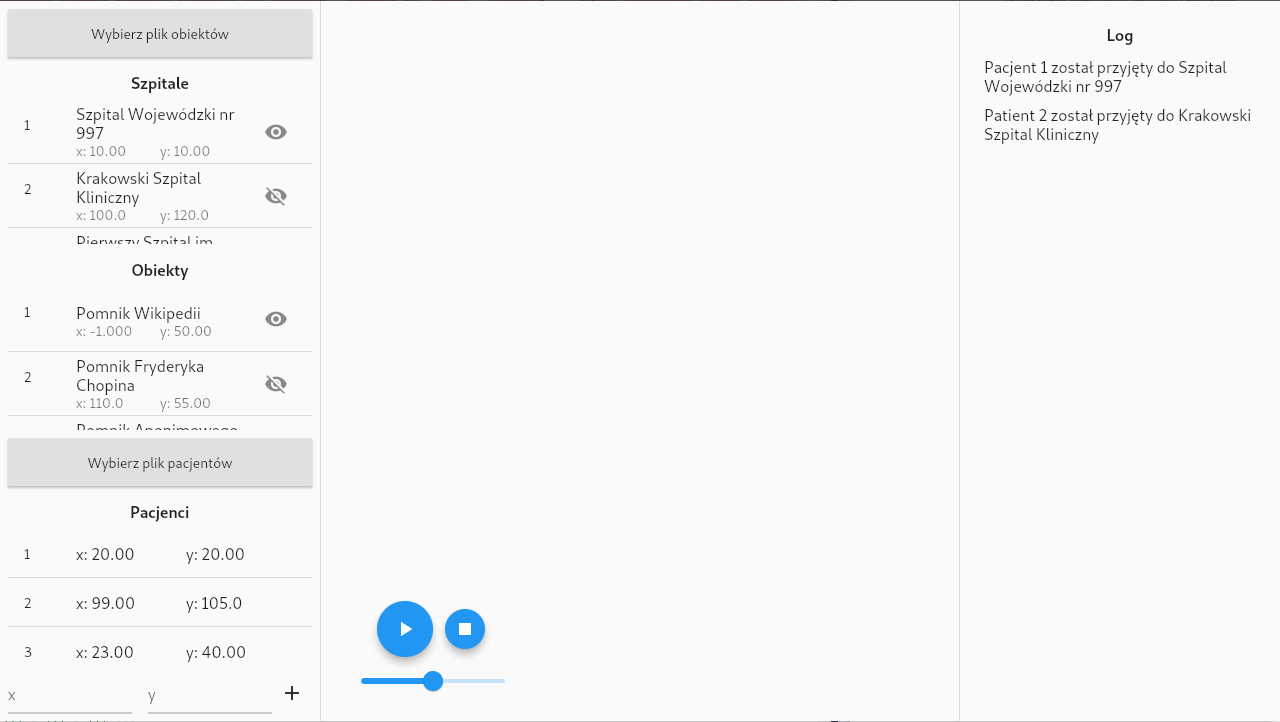
\includegraphics[scale=0.3]{main_page.png}
\caption{Strona główna}
\end{figure}

\section{Testowanie}
Logika biznesowa aplikacji przetestowana zostanie przy użyciu testów jednostkowych napisanych w oparciu o bibliotekę test. Ponieważ zarządzanie stanem aplikacji oparte będzie o architekturę BLoC zostanie ono przetestowane testami jednostkowymi przy pomocy bilibioteki bloc\_test. Interfejs użytkonika przetestowny zostanie manualnie prezez zespół deweloperski.

\newpage
Testowaniu będą podlegały głównie:
\begin{itemize}
    \item Obsługa błędów związanych z niepoprawnymi danymi wejściowymi.
    \item Określanie przez program, czy zgłoszenie pacjenta znajduje się w obszarze działalności szpitala.
    \item Uwzględnianie przez program zajętych miejsc w szpitalach (czy program nie dodaje pacjentów do przepełnionych już szpitali).
    \item Poprawność wyznaczania lokalizacji skrzyżowań.
\end{itemize}

\end{document}
